% sprawozdanie_a3c.tex – szablon w języku polskim
\documentclass[12pt,a4paper]{article}

% ---------------------------------------------------------------
% ↓ PAKIETY ↓
% ---------------------------------------------------------------
\usepackage[utf8]{inputenc}
\usepackage[T1]{fontenc}
\usepackage[polish]{babel}
\usepackage{lmodern}
\usepackage{microtype}

\usepackage{amsmath, amssymb}
\usepackage{graphicx}
\usepackage{booktabs}
\usepackage{siunitx}        % 1\,e\textsuperscript{-3} itp.
\usepackage{hyperref}
\usepackage{caption}
\usepackage{subcaption}
\usepackage{algorithm}
\usepackage[noend]{algpseudocode}

\usepackage{geometry}
\geometry{margin=2.5cm}

\hypersetup{
  colorlinks=true,
  linkcolor=blue,
  citecolor=blue,
  urlcolor=blue
}

% Makro pomocnicze
\newcommand{\E}{\mathbb{E}}
\newcommand{\grad}{\nabla}

\title{\textbf{Asynchroniczny algorytm Advantage Actor–Critic (A3C)\\
dla gry \emph{Pong}}\\
\large{Sprawozdanie z projektu – przedmiot „Algorytmy optymalizacji”}}
\author{Adrian Galik Nr albumu: 268864}
\date{\today}

\begin{document}
\maketitle
\tableofcontents
\clearpage

% ---------------------------------------------------------------
\section{Wprowadzenie}
% ---------------------------------------------------------------

Gry wideo z rodziny Atari stały się w ostatniej dekadzie
\emph{bench­markiem} dla algorytmów uczenia ze wzmocnieniem (RL), ponieważ
łączą dużą przestrzeń stanów (surowe piksele) z niewielką liczbą dyskretnych
akcji oraz wyraźnie zdefiniowaną funkcją nagrody.
Celem niniejszego projektu jest zbudowanie i przeanalizowanie
\textbf{asynchronicznego algorytmu Advantage Actor–Critic (A3C)} oraz jego
\textbf{synchronicznego odpowiednika A2C}, a następnie porównanie obu metod
na przykładzie gry \texttt{PongNoFrameskip-v4}.

\bigskip
\noindent
W szczególności skupiamy się na aspektach \textbf{optymalizacji}:

\begin{itemize}
  \item\,\textit{Równoległość danych}. \
        A3C wykorzystuje wiele procesów, które równolegle symulują środowisko
        i asynchronicznie aktualizują wspólne parametry sieci,
        podczas gdy A2C sumuje gradienty \emph{synchronicznie}
        po każdym kroku uczenia.
  \item\,\textit{Efektywność obliczeń}. \
        Analizujemy, jak liczba procesów i rozmiar mini-batcha wpływają na
        przepustowość danych (klatki/s) oraz szybkość zbieżności nagrody.
  \item\,\textit{Stabilność uczenia}. \
        Badamy wpływ entropii, klipu gradientu i strategii~$n$-step
        na oscylacje funkcji wartości i polityki.
\end{itemize}


% ---------------------------------------------------------------
\section{Podstawy teoretyczne}
% ---------------------------------------------------------------
\label{sec:teoria}

W niniejszym rozdziale streszczamy niezbędne podstawy teorii uczenia ze wzmocnieniem (RL) w ujęciu książki Lapana \cite{Lapan2018} oraz oryginalnego artykułu A3C \cite{Mnih2016A3C}.
Skupiamy się na elementach istotnych z punktu widzenia
\emph{optymalizacji asynchronicznej}.

\subsection{Model formalny RL}

Środowisko opisujemy procesem MDP
$\mathcal{M}=\langle\mathcal{S},\mathcal{A},P,r,\gamma\rangle$,
gdzie $\mathcal{S}$ i $\mathcal{A}$ to odpowiednio przestrzeń stanów
i akcji, $P(s'|s,a)$ – funkcja przejścia, a
$r:\mathcal{S}\times\mathcal{A}\to\mathbb{R}$ – natychmiastowa nagroda.
Agent, obserwując stan $s_t$, wybiera akcję
$a_t\sim\pi_\theta(\cdot|s_t)$
(\emph{polityka})
otrzymuje nagrodę $r_t$ i przechodzi do stanu $s_{t+1}$.
Celem jest maksymalizacja zdyskontowanej sumy nagród
\[
  R_t=\sum_{k=0}^\infty \gamma^{k}r_{t+k},
  \qquad \gamma\in(0,1).
\]
Wartość stanu i wartość akcji definiujemy następująco:
\[
  V^{\pi}(s)=\E_{\pi}[R_t\mid s_t=s],
  \qquad
  Q^{\pi}(s,a)=\E_{\pi}[R_t\mid s_t=s,a_t=a].
\]

\subsection{Gradient polityki i aktor–krytyk}

Twierdzenie o gradiencie polityki
% \cite{Sutton1999policygradient,Lapan2018}
pozwala zapisać pochodną funkcji celu
$J(\theta)=\E_{s\sim d^{\pi_\theta}}\E_{a\sim\pi_\theta}[R_t]$
w postaci:
\begin{equation}
  \grad_\theta J(\theta)=
  \E_{s,a\sim\pi_\theta}
  \bigl[\grad_\theta\!\log\pi_\theta(a|s)\,Q^{\pi_\theta}(s,a)\bigr].
  \label{eq:pg}
\end{equation}
Aktor–krytyk wprowadza aproksymację funkcji $Q$ za pomocą
krytyka $V_w(s)$ oraz \emph{advantage}
$A^{\pi}(s,a)=Q^{\pi}(s,a)-V^{\pi}(s)$, co zmniejsza wariancję estymatora gradientu.

\subsection{n-krokowa aktualizacja}

Zamiast pojedynczego kroku TD, A3C wykorzystuje
$n$-krokowy zwrot
% \cite{Lapan2018}
:
\[
  R^{(n)}_t
  =\sum_{k=0}^{n-1}\gamma^{k}r_{t+k}
   +\gamma^{n}V_w(s_{t+n}),
\]
na podstawie którego definiujemy
\[
  A^{(n)}_t
  =R^{(n)}_t-V_w(s_t).
\]
Wspólny gradient dla parametrów aktora i krytyka wynosi
\begin{align}
  g_\theta &= \grad_\theta\!\log\pi_\theta(a_t|s_t)\,A^{(n)}_t,\\
  g_w      &= \grad_w \tfrac12\bigl(R^{(n)}_t-V_w(s_t)\bigr)^{2}.
\end{align}

\subsection{Synchroniczny A2C a asynchroniczny A3C}

\paragraph{A2C (Advantage Actor–Critic).}
Kilka procesów zbiera dane równolegle, lecz po każdym
mini-batchu \emph{blokująco} agreguje gradienty i wykonuje
wspólny krok optymalizatora („data parallel\,–\,synchronous”).

\paragraph{A3C (Asynchronous A\textsuperscript{3}C).}
Każdy worker oblicza gradient
zaraz po zebraniu własnego mini-batcha
i \emph{natychmiast} aktualizuje wspólne wagi w pamięci RAM
% (\emph{Hogwild!} style) \cite{Mnih2016A3C}.
Skutkuje to brakiem bariery synchronizacji i prawie liniowym wzrostem
przepustowości przy zwiększaniu liczby rdzeni.

\paragraph{Równoległość na poziomie danych vs gradientów.}
W naszej implementacji stosujemy wyłącznie
\emph{data parallelism}: każdy proces:
\begin{enumerate}
  \item symuluje środowisko na CPU,
  \item liczy gradient na CPU,
  \item wysyła gradient do głównego procesu (GPU) lub
        bezpośrednio modyfikuje współdzielone parametry.
\end{enumerate}
Nie używamy równoległości gradientów
(\emph{model parallelism}),
gdyż dysponujemy pojedynczą kartą RTX 2080; kopiowanie tensora
między kilkoma GPU byłoby bardziej kosztowne niż zysk z równoległości.

\subsection{Funkcja straty}

Całkowita funkcja straty używana w eksperymencie, zgodnie
z
% ~\cite{Mnih2016A3C,Lapan2018}
, to
\begin{equation}
  \mathcal{L}
  = -\,\E\!\left[\log\pi_\theta(a_t|s_t)\,A^{(n)}_t\right]
    +c_v\,\E\!\left[\bigl(R^{(n)}_t-V_w(s_t)\bigr)^2\right]
    -\beta\,\mathcal{H}\!\left(\pi_\theta(\cdot|s_t)\right),
\end{equation}
gdzie $c_v$ to współczynnik części wartości (przyjmujemy~$1$),
zaś $\beta$ ($=$\texttt{ENTROPY\_BETA}) kontroluje siłę
regularizacji entropijnej $\mathcal{H}$.

\bigskip
Zestaw wzorów i założeń przedstawiony w tym rozdziale stanowi podstawę
implementacji opisanej w rozdziale~\ref{sec:algorithms}
oraz eksperymentów porównujących wersję synchroniczną (A2C)
i asynchroniczną (A3C).


% ---------------------------------------------------------------
\section{Środowisko \texttt{PongNoFrameskip-v4}}
% ---------------------------------------------------------------
\label{sec:pong}

\texttt{PongNoFrameskip-v4} pochodzi z pakietu \emph{Arcade Learning
Environment} (ALE) i stanowi klasyczny benchmark dla algorytmów RL  
\cite{Mnih2016A3C,Lapan2018}.  
Jest to dwuwymiarowa gra ping-pong, w której agent steruje paletką
po lewej stronie ekranu, a rywal (sterowany przez silnik gry) -
po prawej.  
Agent otrzymuje nagrodę $+1$ po zdobyciu punktu, $-1$ po jego stracie,
w przeciwnym razie $0$.

\subsection{Surowa przestrzeń obserwacji i akcji}

\begin{itemize}
  \item \textbf{Obserwacja} – pojedyncza klatka RGB
        o rozdzielczości \(210\times160\times3\)~px  
        (typ \texttt{uint8}, zakres \([0,255]\)).
  \item \textbf{Akcje} – dyskretny zbiór  
        \(\mathcal{A}=\{0,1,2,3,4,5\}\), gdzie zgodnie z ALE:
        \begin{center}
          \begin{tabular}{cl}
            0 & \texttt{NOOP} \\ 1 & \texttt{FIRE} \\
            2 & \texttt{UP}   \\ 3 & \texttt{RIGHT} \\
            4 & \texttt{LEFT} \\ 5 & \texttt{DOWN}
          \end{tabular}
        \end{center}
  \item \textbf{Epilog gry} – mecz kończy się, gdy jedna ze stron
        zdobędzie \(21\) punktów (maks.\ zwrot $\pm21$).
\end{itemize}

\subsection{Pipeline przetwarzania danych}

Aby zmniejszyć wymiar wejścia i ustabilizować uczenie, stosujemy
standardowy zestaw wrapperów zalecany w \cite{Mnih2016A3C,Lapan2018}:

\begin{enumerate}
  \item \textbf{\texttt{MaxAndSkipEnv} (skip=4)}  
        – wykonuje tę samą akcję przez cztery klatki i zwraca maksimum
        piksel-po-pikselu z dwóch ostatnich; zmniejsza migotanie i 
        przyspiesza symulację \(\approx 4\times\).
  \item \textbf{\texttt{FireResetEnv}}  
        – po resecie wysyła akcje \texttt{FIRE}, aby rozpocząć grę.
  \item \textbf{\texttt{ProcessFrame84}}  
        – konwersja do skali szarości, resize do \(84\times84\)px.
  \item \textbf{\texttt{ImageToPyTorch}}  
        – zmiana kolejności kanałów z~HWC na~CHW (wymóg PyTorch).
  \item \textbf{\texttt{FrameStack} (k=4)}  
        – konkatenacja czterech kolejnych klatek
        \(\Rightarrow\) obserwacja \((4,84,84)\), pozwala
        sieci odtworzyć prędkość piłki.
  \item \texttt{(opc.) \textbf{ScaledFloatFrame}}  
        – dzieli piksele przez 255, zamienia \texttt{uint8} → \texttt{float32}.
\end{enumerate}

Efektem jest końcowy tensor
\begin{equation}
  s_t \in \mathbb{R}^{4\times84\times84},\quad s_t\in[0,1].
\end{equation}

\subsection{Metryki używane w~eksperymentach}

\begin{itemize}
  \item \textbf{Reward per game} –
        suma nagród od rozpoczęcia do końca meczu;
        wartość docelowa \(\ge 18\) punktów
        (\texttt{REWARD\_BOUND} w~kodzie).
  \item \textbf{Frames per second (FPS)} –
        przepustowość danych (kl./s) liczona jako
        liczba przetworzonych klatek/sekundę na CPU.
        Służy do porównania A2C (synchron.) i A3C (asynchron.).
\end{itemize}

\begin{figure}[h]
  \centering
  % \includegraphics[width=0.7\linewidth]{figures/preprocessing_pipeline.pdf}
  \caption{Schemat przetwarzania klatki w pipeline’ie A3C.}
  \label{fig:pipeline}
\end{figure}

\subsection*{Podsumowanie}

Przedstawiony pipeline zmniejsza wymiar wejścia
ponad 10-krotnie i eliminuje zbędne informacje kolorystyczne,
pozwalając sieci konwolucyjnej skupić się na ruchu piłki i paletki.
W dalszych rozdziałach wykorzystujemy identyczny preprocessing
zarówno dla A2C, jak i A3C, aby porównanie było rzetelne.


% ---------------------------------------------------------------
% ---------------------------------------------------------------
\section{Algorytm A3C}
\label{sec:algorithms}

Algorytm \textbf{Asynchronous Advantage Actor–Critic} (A3C)
zaproponowany przez Mniha i wsp. \cite{Mnih2016A3C}
łączy trzy idee:
\begin{enumerate}
  \item gradient polityki z funkcją advantage (aktor–krytyk),
  \item estymację $n$-krokową zwrotu,
  \item równoległe, \emph{asynchroniczne} aktualizacje wspólnych wag.
\end{enumerate}

\subsection{Architektura sieci}
\label{sec:arch}

Zgodnie z~\cite{Mnih2016A3C,Lapan2018} używamy
architektury widocznej na rys.~\ref{fig:net}:
\begin{itemize}
  \item część konwolucyjna wspólna dla polityki i krytyka:  
        \(\mathrm{Conv}_{8,4,32}\rightarrow\)
        \(\mathrm{Conv}_{4,2,64}\rightarrow\)
        \(\mathrm{Conv}_{3,1,64}\rightarrow\)
        \(\mathrm{Flatten}\rightarrow\mathrm{FC}_{512}\),
  \item \textbf{głowa polityki} – warstwa w pełni połączona
        \(\mathrm{FC}_{n_\text{actions}}\) (logity),
  \item \textbf{głowa wartości} – \(\mathrm{FC}_{1}\).
\end{itemize}

\begin{figure}[h]
  \centering
  % \includegraphics[width=.85\linewidth]{figures/a3c_net.pdf}
  \caption{Architektura sieci A3C: wspólny ekstraktor cech
           + dwie głowice (policy, value).}
  \label{fig:net}
\end{figure}

\subsection{$\boldsymbol{n}$-krokowy zwrot i advantage}

Dla każdego stanu $s_t$ i akcji $a_t$ obliczamy
\[
  R^{(n)}_t
    =\sum_{k=0}^{n-1}\gamma^{k}r_{t+k}
     +\gamma^{n}V_w(s_{t+n}),
  \quad
  A^{(n)}_t
    =R^{(n)}_t - V_w(s_t).
\]
Na tej podstawie wyznaczamy gradienty
$g_\theta$, $g_w$ zgodnie z~(\ref{eq:pg})
i formułą entropijną
(\ref{eq:total_loss}).

\subsection{Mechanika asynchroniczna}

Każdy proces–worker:
\begin{enumerate}
  \item pobiera aktualne wagi \(\theta, w\) (w~RAM),
  \item zbiera $n$ kroków trajektorii,
  \item liczy gradient \((g_\theta, g_w)\) lokalnie na CPU,
  \item \emph{bez blokady} dodaje je do wspólnego wektora wag,
  \item zeruje licznik i powtarza.
\end{enumerate}
Brak bariery synchronizacyjnej sprawia, że
złożoność czasowa jednej iteracji $\approx
\frac{\text{czas symulacji}+ \text{backward}}{N_\text{proc}}$,
co przyśpiesza uczenie prawie liniowo z~liczbą rdzeni
(jak pokazują wyniki w~rozdz.~\ref{sec:results}).

\subsection{Pseudokod}

\begin{algorithm}[h]
  \caption{Asynchroniczny worker A3C (wersja CPU)}
  \label{alg:a3c_worker}
  \begin{algorithmic}[1]
  \Require wspólne wagi $\theta, w$, krok optymalizatora \textit{opt}
  \State $t\gets 0$
  \While{nieosiągnięto \textit{max\_frames}}
      \State $s \gets$ \textit{env.reset()}
      \Repeat
          \State $a \sim \pi_\theta(\cdot|s)$
          \State $(s',r,\textit{done})\gets\textit{env.step}(a)$
          \State bufor $\gets$ bufor $\cup\,(s,a,r)$
          \State $t \gets t+1$
          \If{$\textit{done}$ \textbf{or} $|$bufor$|=n$}
              \If{\textit{done}}
                  \State $R\gets 0$
              \Else
                  \State $R\gets V_w(s')$
              \EndIf
              \For{elementy bufora od końca}
                  \State $R \gets r_i + \gamma R$
                  \State $g_\theta += \grad_\theta \log\pi_\theta(a_i|s_i)\,(R-V_w(s_i))$
                  \State $g_w += \grad_w \tfrac12(R-V_w(s_i))^{2}$
              \EndFor
              \State \textbf{atomically} \textit{opt.step}$(g_\theta,g_w)$
              \State wyzeruj bufor
          \EndIf
          \State $s\gets s'$
      \Until{\textit{done}}
  \EndWhile
  \end{algorithmic}
\end{algorithm}

\subsection{Konfiguracja CPU/GPU w implementacji}

W~praktycznej implementacji:
\begin{itemize}
  \item sieć w~workerach działa na \textbf{CPU}  
        (\texttt{torch.set\_num\_threads(1)}), redukując
        przełączanie kontekstu GPU,
  \item wagi współdzielone są w pamięci \texttt{share\_memory()},
  \item główny proces konsoliduje gradienty i kopiuje model
        na GPU wyłącznie do etapu aktualizacji (batch~128).
\end{itemize}

Takie podejście spełnia zalecenia Lapana \cite{Lapan2018}
i pozwala efektywnie wykorzystać pojedynczą kartę RTX~2080,
zachowując zalety asynchronicznej aktualizacji A3C.


% ---------------------------------------------------------------
\section{Konfiguracja eksperymentu}
\begin{itemize}
  \item Sprzęt: Intel i7-7820X (8C/16T), GPU RTX 2080, 16GB RAM
  \item Oprogramowanie: Python 3.12.7, PyTorch 2.5.1, Gymnasium 1.0.0
  \item Hiperparametry: tabela \ref{tab:hparams}
\end{itemize}

\begin{table}[h]
  \centering
  \caption{Kluczowe hiperparametry}
  \label{tab:hparams}
  \begin{tabular}{@{}ll@{}}
    \toprule
    Parametr & Wartość \\ \midrule
    Współczynnik \(\gamma\) & 0{,}99 \\
    Szybkość uczenia (\( \alpha \)) & \(1\cdot10^{-3}\) \\
    Entropy \(\beta\) & 0{,}01 \\
    Liczba procesów & 8 (testy 8-16) \\
    Liczba środowisk / proces & 4 \\ 
    \(n\)-krok & 4 \\ 
    Mini-batch & 128 \\ 
    \bottomrule
  \end{tabular}
\end{table}

% ---------------------------------------------------------------
\section{Wyniki}
% ---------------------------------------------------------------
Poniższe wykresy prezentują przebieg uczenia dla
\textbf{A2C (synchronicznego)} i \textbf{A3C (asynchronicznego)}.
Oba eksperymenty uzyskały podobną liczbę kroków treningowych
(\(\approx10{,}4\) M dla A2C vs \(\approx9{,}2\) M dla A3C);
główna różnica dotyczy \emph{tempa} generowania danych
i szybkości zbieżności.

\begin{figure}[H]
  \centering
  % --- nagrody ---
  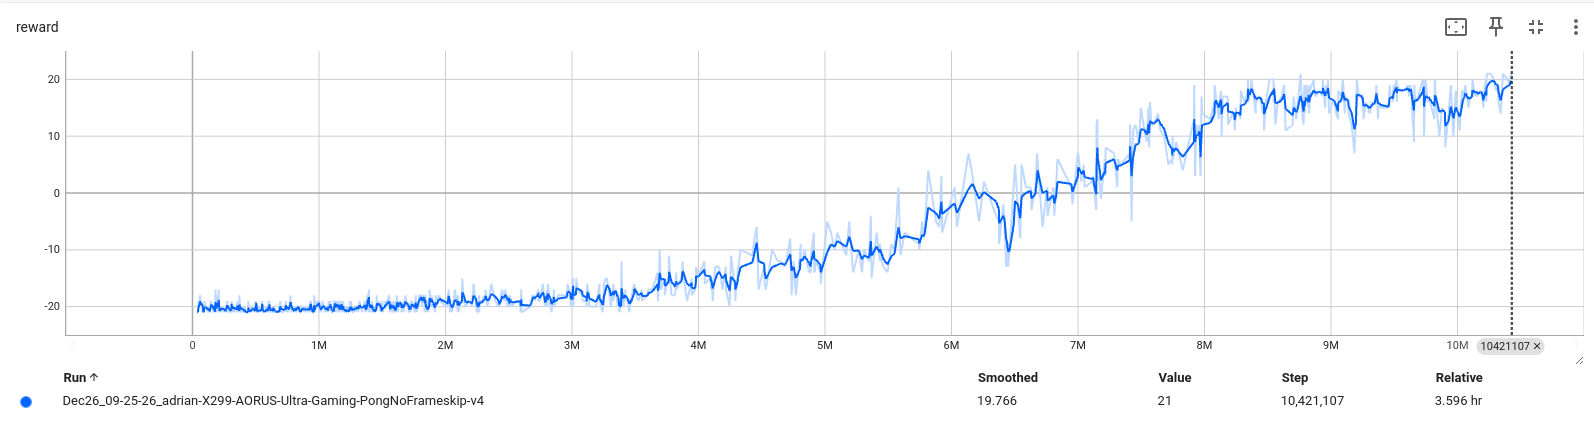
\includegraphics[width=.9\linewidth]{images/A2C_reward.png}
  \caption{A2C – przebieg nagrody w czasie uczenia.}
  \label{fig:a2c_reward}
\end{figure}

\begin{figure}[H]
  \centering
  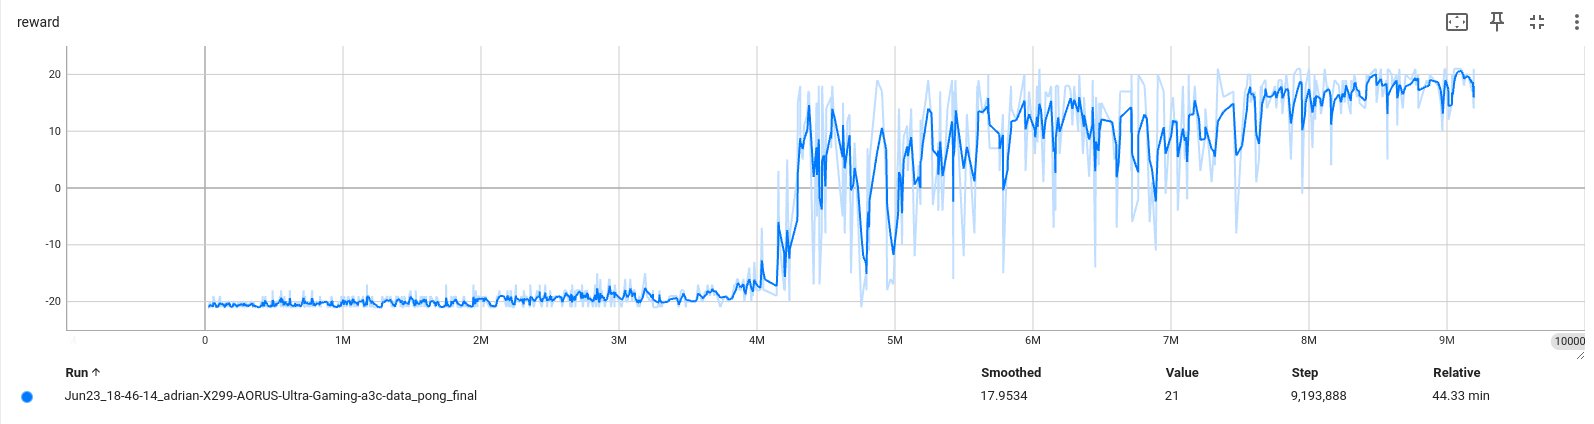
\includegraphics[width=.9\linewidth]{images/A3C_reward.png}
  \caption{A3C – przebieg nagrody w czasie uczenia. Duża wariancja
           wynika z asynchronicznych, częstszych aktualizacji.}
  \label{fig:a3c_reward}
\end{figure}

\begin{figure}[H]
  \centering
  % --- szybkość ---
  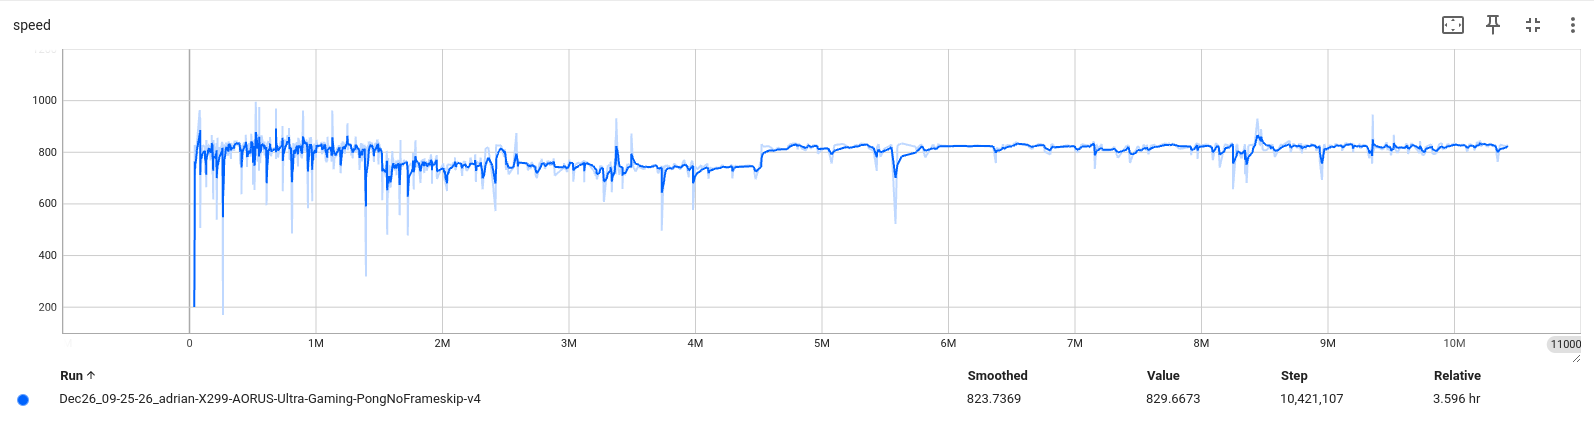
\includegraphics[width=.9\linewidth]{images/A2C_speed.png}
  \caption{A2C – szybkość symulacji (kl./s)}
  \label{fig:a2c_speed}
\end{figure}

\begin{figure}[H]
  \centering
  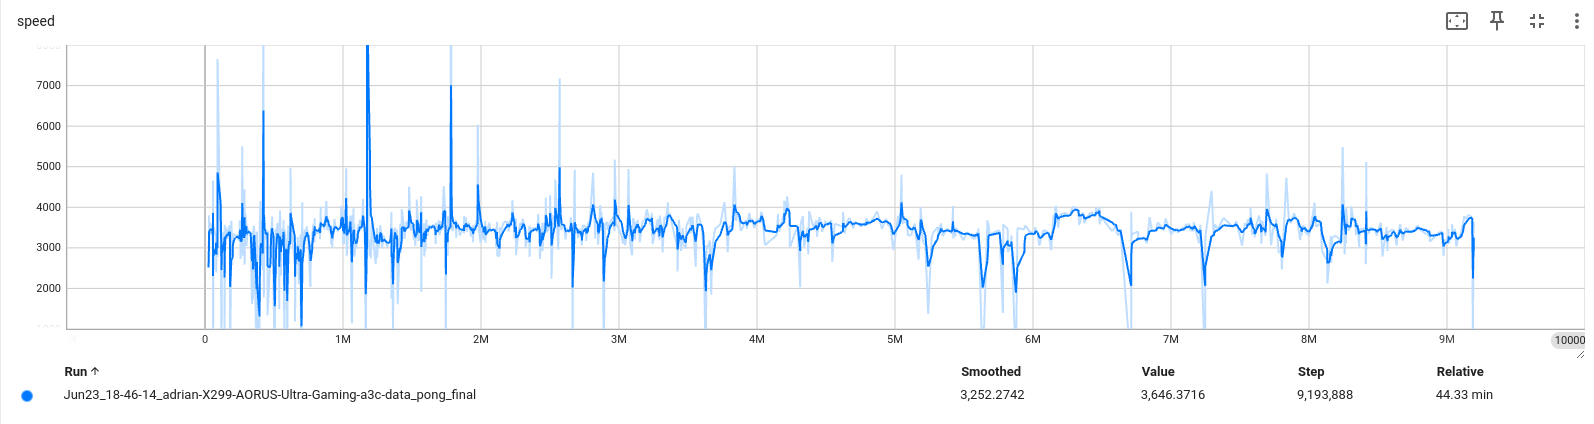
\includegraphics[width=.9\linewidth]{images/A3C_speed.png}
  \caption{A3C – szybkość symulacji (kl./s)}
  \label{fig:a3c_speed}
\end{figure}

\subsection{Porównanie czasu treningu}

\begin{table}[H]
  \centering
  \caption{Czas rzeczywisty potrzebny do osiągnięcia progu
           \(\texttt{REWARD\_BOUND}=18\).}
  \label{tab:time_to_bound}
  \begin{tabular}{@{}lcc@{}}
    \toprule
                 & Czas [hh:mm] & FPS (średnie) \\ \midrule
    A2C          & 03:36        &  \(\approx 800\) \\
    A3C          & 00:45        &  \(\approx 3{,}500\) \\ \bottomrule
  \end{tabular}
\end{table}

Mimo podobnej liczby klatek, A3C osiąga granicę nagrody
\textbf{czterokrotnie szybciej} w czasie rzeczywistym, dzięki wyższej przepustowości
CPU.
Jest to bezpośredni efekt większej przepustowości symulacji
oraz częstszych, choć bardziej hałaśliwych aktualizacji wag.

\subsection{Wariancja nagrody}

Krzywa nagrody A3C (Rys.~\ref{fig:a3c_reward})
wykazuje znacznie wyższą wariancję niż A2C.
Źródła zjawiska:

\begin{enumerate}
  \item \textbf{Asynchroniczne opóźnienie gradientu}.  
        W momencie gdy jeden worker modyfikuje wspólne wagi,
        pozostałe procesy wciąż mogą liczyć gradient
        względem \emph{starej} wersji sieci,
        co wprowadza stochastyczny „szum aktualizacji”.
  \item \textbf{Mniejszy $n$-batch lokalny}.  
        Każdy worker A3C propaguje gradient co 32 próbki
        (\texttt{MICRO\_BATCH\_SIZE}), podczas gdy
        A2C kumuluje pełne batche 128 elementów
        przed jednym, synchronicznym krokiem.
  \item \textbf{Różnica w $n$-kroku}.  
        $n=4$ w A3C oznacza dłuższy horyzont bootstrapu,
        a więc wyższą wariancję celu $R^{(n)}$ w porównaniu
        z~$n=3$ w A2C.
\end{enumerate}

Mimo większych odchyleń, średnia krocząca A3C
zbiega szybciej i stabilizuje się w~obszarze \( \approx 19\text{–}21\)
punktów (nagroda maksymalna dla \emph{Ponga}).

\subsection{Analiza efektywności}

\begin{itemize}
  \item \textbf{Wydajność CPU}.  
        Dzięki \texttt{PROCESSES\_COUNT}=8 i
        \texttt{NUM\_ENVS}=4 wykorzystujemy 32 lekkie środowiska,
        co saturuje wszystkie 8 rdzeni fizycznych
        (HT: 16 wątków) i przekłada się na
        \(\sim3{,}5\)k~kl./s.
  \item \textbf{Koszt synchronizacji}.  
        A2C traci czas na barierę zbierania gradientów:
        FPS ustala się na \(\sim 800~kl./s\) mimo
        50 środowisk (\texttt{NUM\_ENVS}=50) — koszt kopiowania
        dużego batcha na GPU co krok.
  \item \textbf{Zużycie GPU}. 
        Podczas trenowania algorytmu A2C zużycie GPU było na poziomie \(\sim 40\)\%,
        natomiast dla A3C dzięki wykorzystaniu synchroniczności osiągnęło \(\sim 80 \)\%.
\end{itemize}

\subsection*{Wnioski z eksperymentu}

\begin{enumerate}
  \item A3C znacząco redukuje czas treningu na sprzęcie CPU + jedna GPU,
        wykorzystując proste zrównoleglenie na poziomie danych
        i brak bariery synchronizacji.
  \item Wyższa wariancja nagrody to efekt
        „starych” gradientów i mniejszych batchy,
        lecz nie pogarsza końcowej wydajności agenta.
  \item Przy zwiększaniu liczby procesów
        warto jednocześnie podnieść rozmiar globalnego batcha
        lub obniżyć \(\alpha\), aby uniknąć zbyt gwałtownych
        oscylacji wartości krytyka.
\end{enumerate}

% ---------------------------------------------------------------
\bibliographystyle{plplain}  % lub inny styl obsługujący jęz. polski
\bibliography{refs}



\end{document}
